% =========================================================================
% Academic Book Cover Architect - Outer Cover (Full-Bleed 6x9 in, 2:3 Ratio)
% Featuring Asst. Prof. Dr. Chewa Thassana, Plasma N2 Fixation & Green Urea
% Large 2.5x Multicolor Title: พลาสมาฟิสิกส์ (55pt)
% =========================================================================

\definecolor{specViolet}{HTML}{6B21A8} % Deep Electric Purple-Violet
\definecolor{specCyan}{HTML}{0284C7}   % Vivid Deep Cyan
\definecolor{specEmerald}{HTML}{047857} % Deep Emerald Green
\definecolor{specCoral}{HTML}{C2410C}   % Deep Solar Coral-Amber

\begin{titlepage}
\thispagestyle{empty}
\begingroup
\setlength{\XeTeXlinebreakskip}{0pt}
\begin{tikzpicture}[remember picture, overlay]
    % 1. Full-Bleed Cover Artwork (6x9 inch, 2:3 Ratio)
    % Latest Artwork: Atmospheric Nitrogen Fixation to Green Urea & Cold Plasma Agro-Physics
    \node[anchor=center, inner sep=0pt] at (current page.center) {
        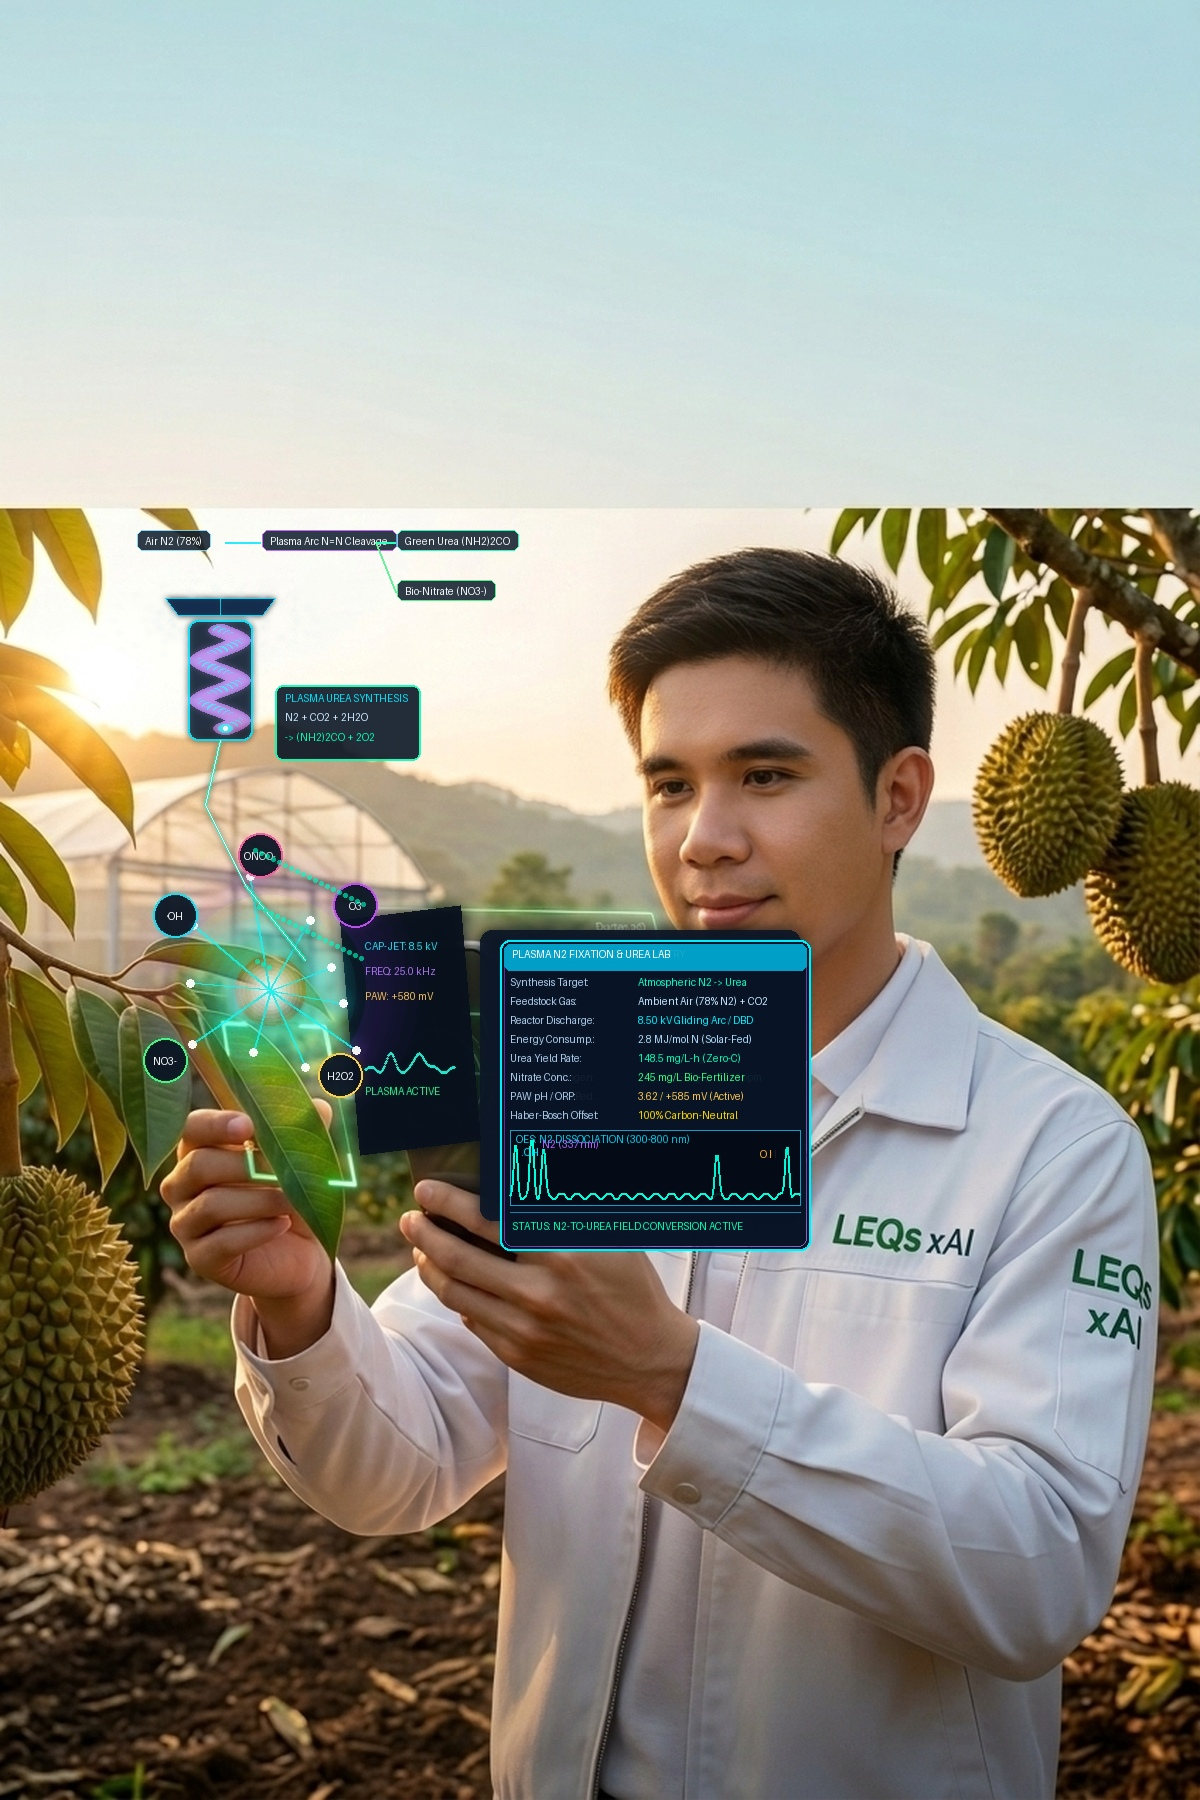
\includegraphics[width=\paperwidth,height=\paperheight]{figures/cover_art_concept_plasma_urea.jpg}
    };

    % 2. UPPER SKY ZONE: Transparent Architecture with Dual-Layer Micro Drop-Shadow
    % Shadow Layer (Soft white glow halo for crisp contrast against pastel morning sky)
    \node[anchor=north, align=center, text width=5.4in] at ([xshift=0.6pt, yshift=-0.076in]current page.north) {
        \begin{tikzpicture}
            \node[fill=deepIndigo!85, text=white, rounded corners=2.5mm, inner sep=3.5pt, font=\fontsize{7.5}{9.5}\selectfont\bfseries] {
                \color{cyberCyan}$\blacktriangleright$\ \color{white}TEXTBOOK SERIES IN APPLIED PHYSICS \& PLASMA AGRICULTURE\ \color{neonEmerald}$\blacktriangleleft$
            };
        \end{tikzpicture}\\[2.5pt]
        {\fontsize{8.5}{11}\selectfont\color{white}\textbf{ตำราวิชาการและคู่มือการวิจัยขั้นสูง \textbullet\ มหาวิทยาลัยราชภัฏรำไพพรรณี}}\\[3pt]
        
        % Main Title Line 1 (2.5x Size = 55pt in Pure White Shadow)
        {\fontsize{55}{62}\selectfont\bfseries\color{white} พลาสมาฟิสิกส์}\\[2pt]
        % Main Title Line 2
        {\fontsize{24}{30}\selectfont\bfseries\color{white} เพื่อการเกษตรและสิ่งแวดล้อม}\\[3.5pt]
        % Subtitle Pill Tag
        \begin{tikzpicture}
            \node[draw=cyberCyan, line width=1.1pt, rounded corners=2.5mm, inner sep=3.5pt] {
                \fontsize{11}{14}\selectfont\bfseries\color{white} จากทฤษฎีสู่นวัตกรรมความยั่งยืน
            };
        \end{tikzpicture}\\[3pt]
        % English Subtitle
        {\fontsize{8.2}{10.5}\selectfont\bfseries\color{white} PLASMA PHYSICS FOR AGRICULTURE AND ENVIRONMENT}\\[1.5pt]
        {\fontsize{7}{9}\selectfont\color{white} (FROM FUNDAMENTAL DISCHARGE PHYSICS TO SUSTAINABLE SMART AGRO-AI INNOVATION)}
    };

    % Foreground Layer (Crisp typography with Multicolored Plasma Spectrum)
    \node[anchor=north, align=center, text width=5.4in] at ([yshift=-0.08in]current page.north) {
        \begin{tikzpicture}
            \node[fill=deepIndigo!92, text=white, rounded corners=2.5mm, inner sep=3.5pt, font=\fontsize{7.5}{9.5}\selectfont\bfseries] {
                \color{cyberCyan}$\blacktriangleright$\ \color{white}TEXTBOOK SERIES IN APPLIED PHYSICS \& PLASMA AGRICULTURE\ \color{neonEmerald}$\blacktriangleleft$
            };
        \end{tikzpicture}\\[2.5pt]
        {\fontsize{8.5}{11}\selectfont\color{deepIndigo!90}\textbf{ตำราวิชาการและคู่มือการวิจัยขั้นสูง \textbullet\ มหาวิทยาลัยราชภัฏรำไพพรรณี}}\\[3pt]
        
        % Main Title Line 1 (2.5x Size = 55pt, Multicolored Plasma Spectrum)
        {\fontsize{55}{62}\selectfont\bfseries%
        {\color{specViolet}พลาส}%
        {\color{specCyan}มา}%
        {\color{specEmerald}ฟิ}%
        {\color{specCoral}สิกส์}%
        }\\[2pt]
        % Main Title Line 2
        {\fontsize{24}{30}\selectfont\bfseries\color{agriGreen!85!black} เพื่อการเกษตรและสิ่งแวดล้อม}\\[3.5pt]
        % Subtitle Pill Tag
        \begin{tikzpicture}
            \node[draw=cyberCyan!90, line width=1.1pt, fill=white!55, fill opacity=0.55, text opacity=1.0, rounded corners=2.5mm, inner sep=3.5pt] {
                \fontsize{11}{14}\selectfont\bfseries\color{deepIndigo} จากทฤษฎีสู่นวัตกรรมความยั่งยืน
            };
        \end{tikzpicture}\\[3pt]
        % English Subtitle
        {\fontsize{8.2}{10.5}\selectfont\bfseries\color{deepIndigo!95} PLASMA PHYSICS FOR AGRICULTURE AND ENVIRONMENT}\\[1.5pt]
        {\fontsize{7}{9}\selectfont\color{deepIndigo!80} (FROM FUNDAMENTAL DISCHARGE PHYSICS TO SUSTAINABLE SMART AGRO-AI INNOVATION)}
    };

    % 3. BOTTOM ZONE: Natural Dark Soil Canvas with Micro Shadow & Soft Depth Vignette
    \shade[top color=transparent, bottom color=black!85, opacity=0.90] 
        ([yshift=0.95in]current page.south west) rectangle (current page.south east);

    % Shadow Layer
    \node[anchor=south, align=center, text width=5.3in] at ([xshift=0.5pt, yshift=0.106in]current page.south) {
        {\fontsize{14}{18}\selectfont\bfseries\color{black!98} ผู้ช่วยศาสตราจารย์ ดร.ชีวะ ทัศนา}\\[2.5pt]
        {\fontsize{9}{12}\selectfont\bfseries\color{black!98} สาขาวิชาปัญญาประดิษฐ์เพื่อเกษตรดิจิทัลและสิ่งแวดล้อม คณะวิทยาศาสตร์และเทคโนโลยี}\\[2pt]
        {\fontsize{8.5}{11}\selectfont\bfseries\color{black!98} มหาวิทยาลัยราชภัฏรำไพพรรณี \textbullet\ พ.ศ. 2569}
    };
    % Foreground Layer
    \node[anchor=south, align=center, text width=5.3in] at ([yshift=0.11in]current page.south) {
        {\fontsize{14}{18}\selectfont\bfseries\color{white} ผู้ช่วยศาสตราจารย์ ดร.ชีวะ ทัศนา}\\[2.5pt]
        {\fontsize{9}{12}\selectfont\bfseries\color{white!98} สาขาวิชาปัญญาประดิษฐ์เพื่อเกษตรดิจิทัลและสิ่งแวดล้อม คณะวิทยาศาสตร์และเทคโนโลยี}\\[2pt]
        {\fontsize{8.5}{11}\selectfont\bfseries\color{techAmber} มหาวิทยาลัยราชภัฏรำไพพรรณี \textbullet\ พ.ศ. 2569}
    };
\end{tikzpicture}
\endgroup
\end{titlepage}
\cleardoublepage
